\documentclass[t]{beamer}
%% option to suppress auto-gen of document properties: usepdftitle=false
\usepackage[english]{babel}
%\usepackage{dcolumn}
\usepackage{bbold}
\usepackage{amsmath}
\usepackage{soul}
\usepackage{appendixnumberbeamer}

\usepackage{booktabs}
\usepackage{tabu}

\usepackage{tikz}
\usetikzlibrary{bayesnet}

\newcommand{\myemph}[1]{\alert{#1}}
\newcommand{\email}[1]{$\langle${#1}$\rangle$}
% \graphicspath{{../matlab/}}
% \newcolumntype{d}[1]{D{.}{.}{#1}}
\usepackage{hyperref}
\definecolor{myBlue}{rgb}{.75,.91,1}
\definecolor{myDarkBlue}{rgb}{0.0,0.0,0.55}
\definecolor{myRed}{rgb}{.698,.132,.132}
\definecolor{BrickRed}{rgb}{.698,.132,.132}
\definecolor{myGreen}{rgb}{.196,.804,.196}
\definecolor{BurntOrange}{rgb}{1,.648,0}
\definecolor{myGrey}{rgb}{.5,.5,.5}
\definecolor{LightCyan}{rgb}{0.88,1,1}

% Use "show notes" or "hide notes"
\setbeameroption{hide notes}

\mode<presentation>
{
  \usetheme{AnnArbor}
  \usecolortheme{default}
  \usefonttheme{default}
  \setbeamercovered{transparent}
  \setbeamerfont{downsize}{size=\footnotesize}
}
\mode<handout>
{
  \usetheme{default}
  \usecolortheme{default}
  \usefonttheme{default}
}
\AtBeginSection[]
{
  \begin{frame}
    \frametitle{Table of Contents}
    \tableofcontents[currentsection]
  \end{frame}
}
\title[Causal Inference in NFL]{What was lost? \\ A causal estimate of fourth down behavior in the National Football League \footnote{https://doi.org/10.3233/JSA-190294}}
\author[Derek Hansen]{Discussant: Derek Hansen}
\institute[UM Statistics]{Sports Reading Group \\ University of Michigan Department of Statistics}
\date{September 25, 2020}
\begin{document}

\frame{\titlepage}

\begin{frame}
  \frametitle{Motivating Example}
  \begin{itemize}
  \item https://youtu.be/fwWoBNELyeU?t=630
  \end{itemize}
  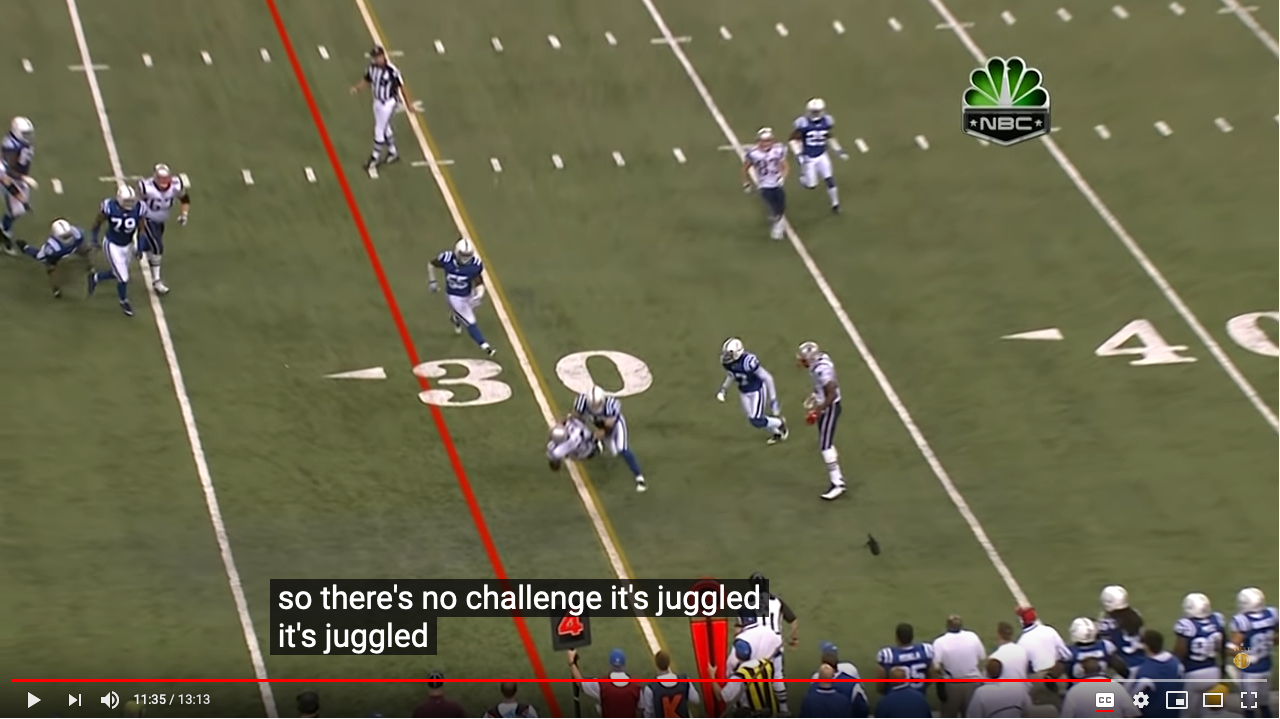
\includegraphics[width=\linewidth]{./motivating_example.png}
\end{frame}

% \begin{frame}
%   \frametitle{Overview}
%   \tableofcontents
% \end{frame}
\begin{frame}
  \frametitle{Background}
  \begin{itemize}
  \item In American football, attempting to convert on fourth-down rather than
    punting or kicking a field-goal is a classic high-risk, high-reward
    decision.
    \item Successful conversion keeps possession and gives the team a chance to score a touchdown
    \item A failed conversion surrenders possession at the current spot on the field, which puts the opposing team in a good position to score.
    \item Did Bill Belichick make the right decision against the Colts in 2009?
  \end{itemize}
\end{frame}

% \begin{frame}
%   \frametitle{Introduction}
%   \begin{itemize}
% \item Unlike in Madden, going for it on fourth down every time is reckless because the risk-reward ratio changes depending on the game scenario, the yards to go, and the position on the field
%   \item If you're losing late in the fourth quarter, makes sense to go for it.
%   \item If you're close to your own endzone, you risk giving the opponent an easy score
%   \item If you're past the 50 yard line but too far for an easy field goal, going for it makes sense because a punt won't improve field position that much and a missed field goal is worse than going for it and not converting.
% \end{itemize}
% \end{frame}


\begin{frame}
  \frametitle{Overview of Paper}
  \begin{itemize}
  \item Previous studies in literature suggest NFL coaches are risk-averse and do not attempt to convert on fourth-down enough.
  \item The New York Times has a 4th Down Bot that gives real-time suggestions on whether a team should attempt to convert or not.
  \item This study focused on plays that the 4th Down Bot said to go for it  \item This study used a matching algorithm based on propensity scores to estimate the difference in win probability if teams had gone for it instead.
   \item They find that the win probability increased in expectation, but also an increase in variance due to a bimodal distribution (confirming the high-risk, high-reward of going for it)
  \end{itemize}
\end{frame}

\begin{frame}
  \frametitle{Past studies}
  \begin{itemize}
  \item Carter and Machol (1978): Teams kick too many field goals (based on
    expected points framework)
  \item Romer (2006): Found that teams were not aggressive enough on fourth down (expected points)
  \item Burke and Quealy (2013): Expanded Romer (2006); authors helped create the NYT's ``4th Down Bot''
  \item Causey et al (2015): Expanded Burke and Qualy to use more data and changed from expected points to win probability in cross-validated logistic regression
  \end{itemize}
\end{frame}

\begin{frame}
  \frametitle{The Coachs' Opinions}
  \begin{itemize}
  \item Despite empirical evidence mostly suggesting coaches are overly conservative, there is no known evidence that coaches' have modified their behavior since 2006.
  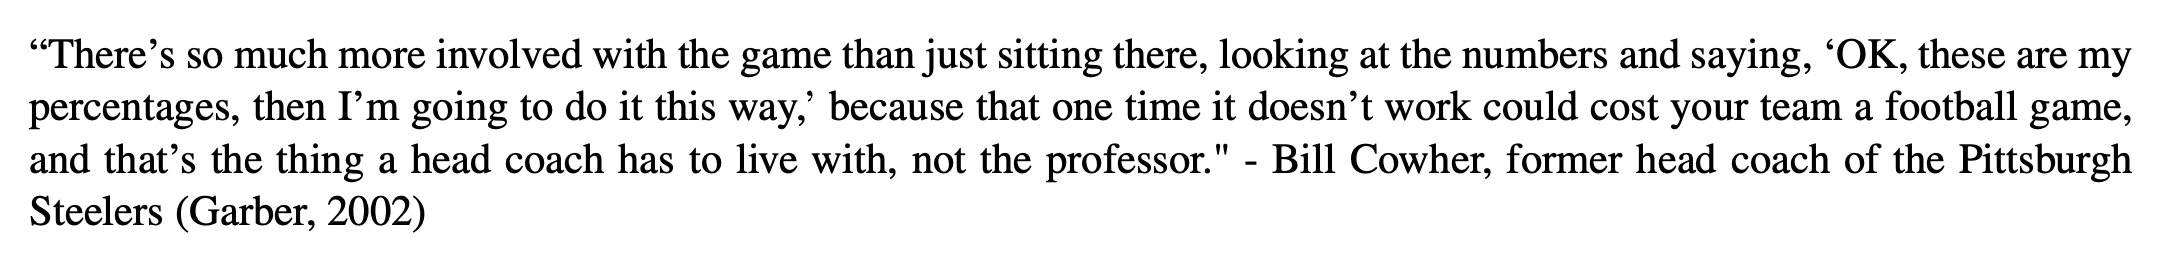
\includegraphics[width=\linewidth]{./cowher.png}
\item ``Analytics is not really my thing. I just try to evaluate what I see.'' - Bill Belichick \footnote{https://www.boston.com/sports/new-england-patriots/2019/09/27/bill-belichick-analytics-patriots-bills}
\item Belichick was also asked how much of a role analytics plays in his decision-making process, specifically in regards to two-point conversions and going for it on fourth down. Belichick responded, “less than zero.”
  \end{itemize}
\end{frame}

\begin{frame}
  \frametitle{Model}
  \begin{itemize}
  \item Each observation is a play where the 4th Down Bot suggests to go for it.
  \item $Y_i$ is the potential change in win probability \footnote{As determined by a pre-trained model discussed in the Appendix. They tried two different models: random forest and GAM.} for the team on offense.
    \begin{itemize}
    \item $Y_i(1)$ is the change in win probability if the team goes for it. (Treatment)
    \item $Y_i(0)$ is the change in win probability if the team opts to kick or punt. (Control)
    \end{itemize}
  \end{itemize}
\end{frame}


\begin{frame}
  \frametitle{Data}
  \begin{itemize}
  \item Data from ArmchairAnalysis.com from 2004 through 2016.
  \item $n=13,172$ fourth downs identified where teams should have gone for it.
  \item $9,348$ teams ($71.0\%$) did not go for it (i.e. the control group), and $3,824$ teams did go for it (i.e. the treatment group)
  \item Removed plays on which a penalty occured.
  \item https://github.com/statsbylopez/nfl-fourth-down for code (although data is behind paywall)
  \end{itemize}
\end{frame}

\begin{frame}
  \frametitle{Model covariates used in win-probability model}
  \centering 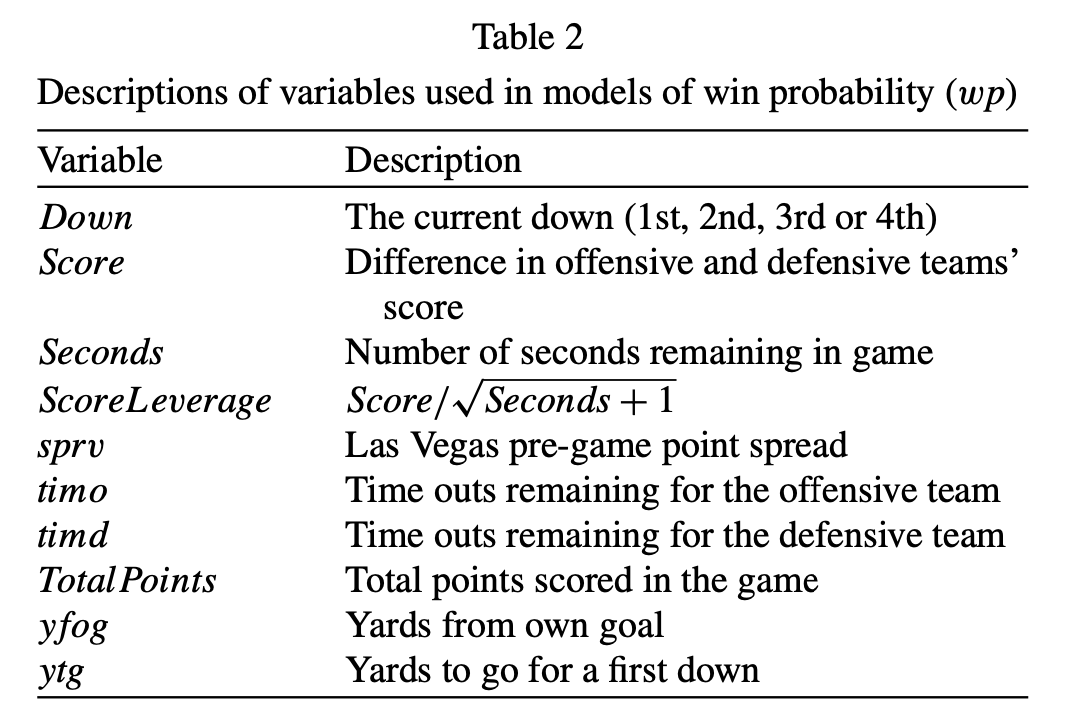
\includegraphics[width=0.8\linewidth]{./covariates_wp.png}
\end{frame}
\begin{frame}

  
  \frametitle{Model- Causal Inference Assumptions}
  \begin{itemize}
  \item Stable unit treatment value assumption (SUTVA) is reasonable for this model
    \begin{itemize}
    \item The potential outcome $Y_i$ does not vary based on treatments assigned to other subjects.
    \item There is no hidden variation of treatment (``decision to go for it is made prior to any play'').
    \end{itemize}
  \item $W_i$ is the assignment of treatment.
  \item $Y_i^{obs} = Y_i(W_i)$ is the observed outcome, $Y_i^{mis} = Y_i(1-W_i)$ is the missing outcome.
   \item $X_i$ are covariates associated with play $i$ (shown in a few slides)
   \item Assume \(P(W_i = 0 | X_i) > 0\) and \(P(W_i=1 | X_i) > 0\).
    \item \textbf{Ignorability}: $P(W | X, Y_i(0), Y_i(1)) = P(W | X)$.
  \end{itemize}
\end{frame}
\begin{frame}
  \frametitle{Average and Team-specific total treatment effects}
  \begin{itemize}
  \item The Average Treatment effect on the Control (ATC) is defined when $W_i = 0$. 
    \[
      \begin{split}
      ATC_i &= Y_i^{mis} - Y_i^{obs} = Y_i(1) - Y_i(0) \\
      ATC  &= \frac 1 {N_c} \sum_{W_i=0} ATC_i\\
    \end{split}
  \]
 \item The Total Treatment effect on the Control for team $f$ ($TTF_f$) is:
   \[
     \begin{split}
       TTC_f = \sum_{i: W_i = 0} ATC_i 1[F_i = f]
     \end{split}
   \]
   where $f = 1, \dots, 32$ are NFL teams and $F_i$ is the team on offense for play $i$.
  \end{itemize}
\end{frame}

\begin{frame}
  \frametitle{Propensity scores}
  \begin{itemize}
  \item Very unlikely to find two plays where $X_i$ is exactly the same
    \item Solution is to match plays with propensity scores, defined as:
      \[
        e(X_i) = P(W_i=1 | X)
      \]
    \item These scores are estimated with a logistic regression model with spline terms for continuous variables, along with some interation terms. (see Table 3 in Appendix)
    \item Propensity scores are filtered out which are above maximum or below the minimum of either the treatment or control group.
  \end{itemize}
\end{frame}

\begin{frame}
  \frametitle{Model covariates used in propensity scores}
  \centering 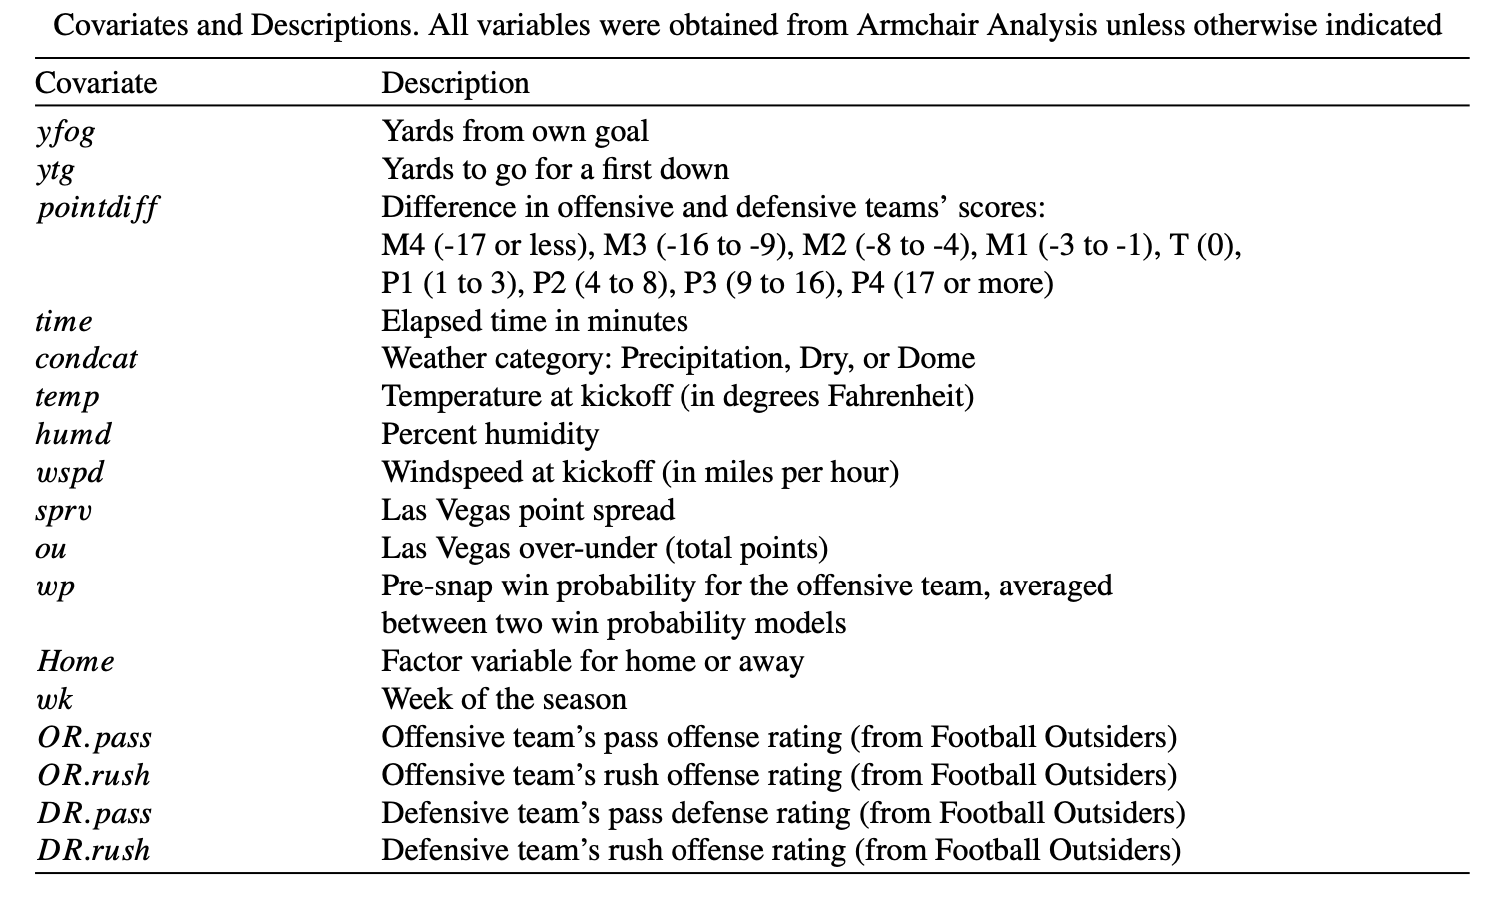
\includegraphics[width=\linewidth]{./covariates.png}
\end{frame}

\begin{frame}
  \frametitle{Matching}
  \begin{itemize}
  \item $1:1$ nearest neightbor matching treatments to the control group using four play characteristics:
    \begin{enumerate}
    \item $\mathrm{logit}(e(X))$ : propensity scores
    \item $\mathrm{logit}(wp)$ : pre-snap win probability
    \item $ytg$ : yards to go
    \item $time$ : number of minutes remaining in the game
    \end{enumerate}
  \item Calipers set to exclude observations that don't have a match which is within a certain threshold for each variable. 
  \end{itemize}
\end{frame}

\begin{frame}
  \frametitle{Matching Performance}
  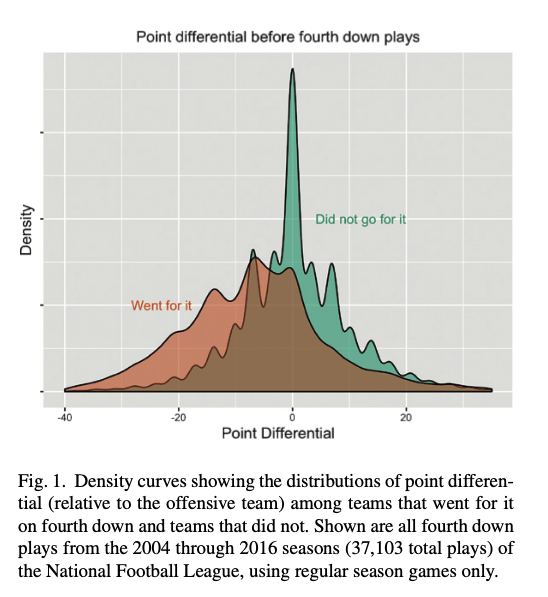
\includegraphics[width=0.4\linewidth]{./pre_matching.png}
  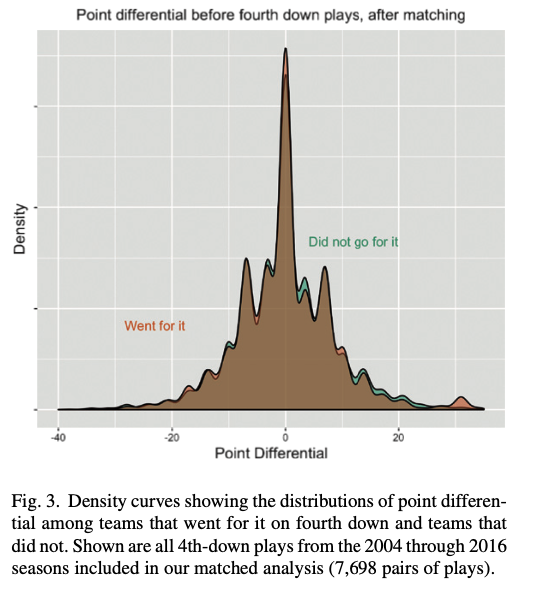
\includegraphics[width=0.4\linewidth]{./post_matching.png}
\end{frame}

\begin{frame}
  \frametitle{Matching Performance}
  \centering 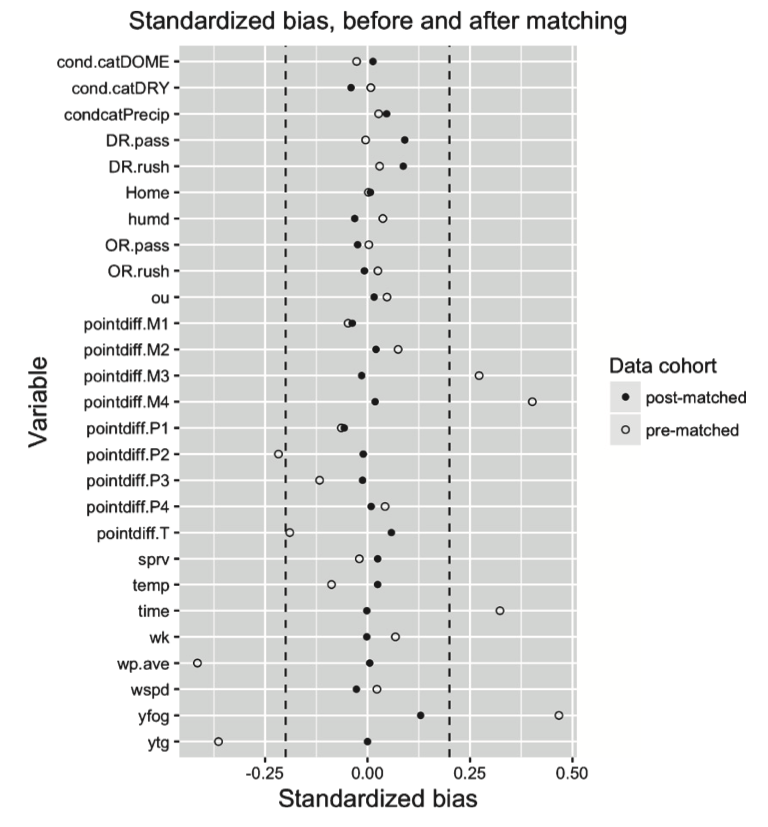
\includegraphics[width=0.55\linewidth]{./love.png}
\end{frame}


\begin{frame}
  \frametitle{Findings}
  \begin{itemize}
  \item Overall, teams that went for it have an average increase in win probability of $1.9 \%$.
  \item The observed distribution of $ATC_i$ was bimodal, corresponding to whether a team is successful or not.
  \end{itemize}
  \centering  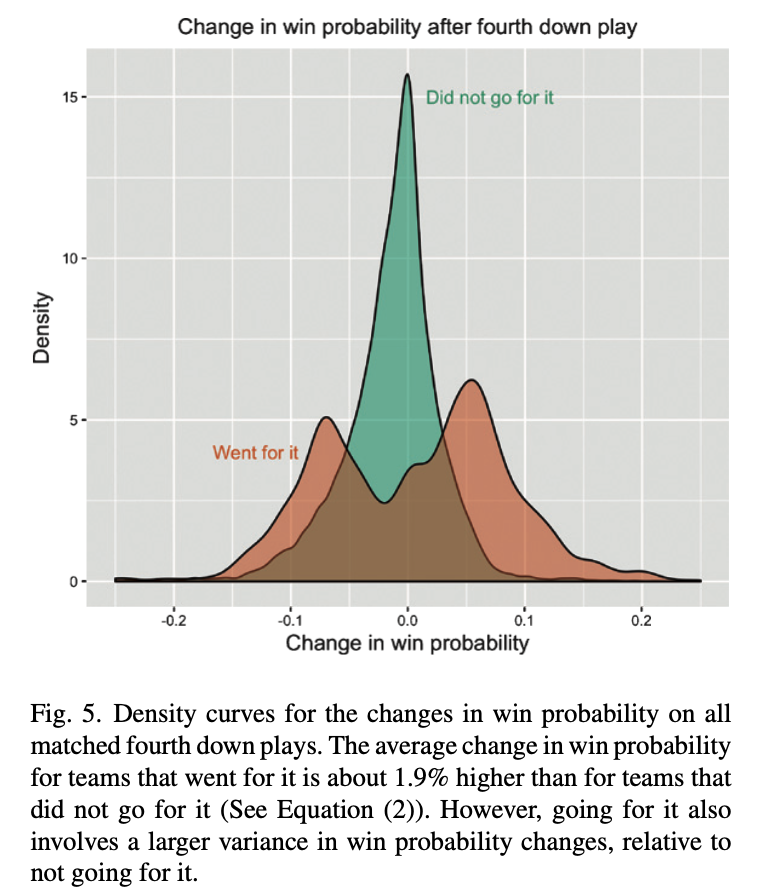
\includegraphics[width=0.4\linewidth]{./change_win_probability.png}
\end{frame}

\begin{frame}
  \frametitle{Findings}
  \begin{column}{0.5\linewidth}
      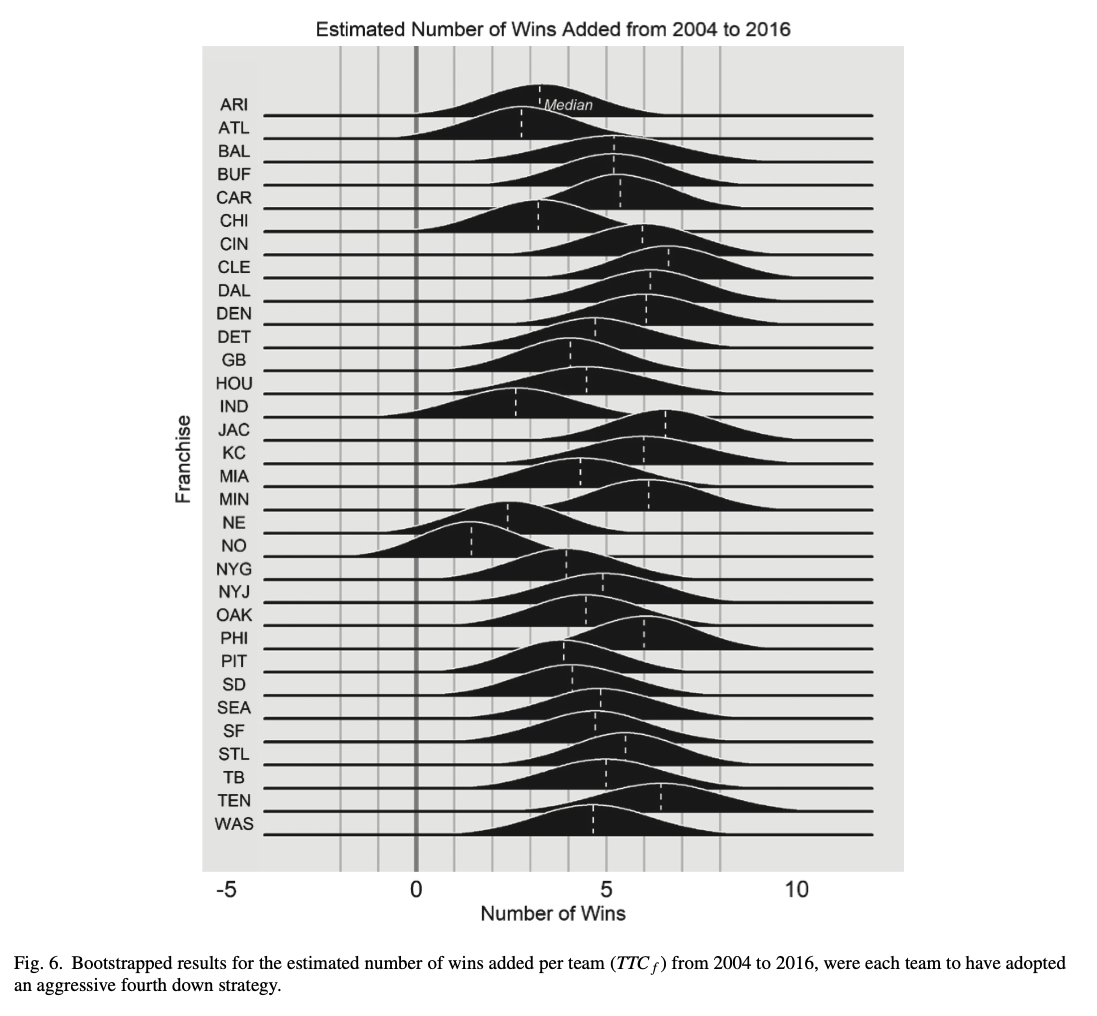
\includegraphics[width=\linewidth]{./team_wins.png} 
    \end{column}
    \begin{column}{0.5\linewidth}
      \begin{itemize}
      \item \small Plot shows estimated change in wins from 2004-2016 if teams always went for it when 4th Down Bot said to (based on matched outcome).
      \item Team with highest number of expected increase in wins is Cleveland with 6.7.
      \item Only for New England, Indianapolis, and New Orleans is it feasible that the more aggresive strategy would not increase win total (matches perceptions that their coaches make better decisions on fourth down)
      \end{itemize}
    \end{column}
\end{frame}
\begin{frame}
  \frametitle{Discussion}
  \begin{itemize}
  \item It would make more sense to group by Head Coaches than Teams to account for differences in philosophy
  \item It's hard to say that a coach isn't able to infer signal about $Y_i(1)$ and $Y_i(0)$ based on variables not in the covariates.
  \end{itemize}
  \end{frame}
  \begin{frame}
      \frametitle{Discussion}
      
      \begin{itemize}
    \item This paper maybe suggests that Bill Belichick was right to go for it on fourth down against the Colts.
      \begin{enumerate}
      \item In 2005 against the Saints, New England faced ``a 4th-and-2, 68 yards from its own goal, 10 minutes into a tied game, and successfully completed a four-yard pass, resulting in a $Y=  \Delta wp = 8.5\%$''.
      \item The increase in winning-percentage if New England had converted, $Y_i(1) | \{\text{converted}\}$, would likely have been higher. Indianapolis had one time-out and it would have been past the 2-minute warning.
      \item With two minutes on the clock, playing against a red-hot Peyton Manning and Reggie Wayne, the difference between $Y_i(1) | \{\text{not converted}\}$ and $Y_i(0)$ might not have been that high.
      \end{enumerate}
    \end{itemize}
    \end{frame}
\end{document}